\typeout{NT FILE IMPLEM.tex}%
\chapter{Implementation}
\label{cha:implementation}
This chapter presents the implementation phase for the \gls{uspfs} and
\gls{sspfs} solutions. We start by outlining the overall implementation
workflow. Then, we present the base system, i.e., the common set of hardware and
software components between the two solutions, where we perform an initial
validation of these components, namely: the \gls{uav} assembly and
configuration, and the PX4 and video surveillance stacks. Next, we implement the
\gls{uspfs} solution by deploying the
PX4 and video surveillance stacks to a custom embedded Linux-based
\gls{os}. Lastly, we implement the \gls{sspfs} solution by deploying each
software stack to its separate \gls{vm}, running atop of the Bao hypervisor.

\section{Workflow}
\label{sec:workflow}
Fig.~\ref{fig:uav-main-Implem-Workflow} illustrates the overall implementation
workflow: the \gls{uspfs} solution comprises the \textbf{Guests}, \textbf{Firmware},
and \textbf{Deployment} sections, and the \gls{sspfs} solution also includes the
\textbf{Hypervisor} section. On the left we can see the four major
implementation's steps: \textbf{Build guests},
\textbf{Build Hypervisor and VMs} (\gls{sspfs} only), \textbf{Build Firmware},
and \textbf{Deployment}. The term ``guest'' is used loosely here, meaning an
actual guest that executes atop of the Bao hypervisor in the \gls{sspfs} case,
or a binary that runs natively on the \gls{uavic} platform (\gls{uspfs}).

\begin{figure}[!hbt]
  \centering
  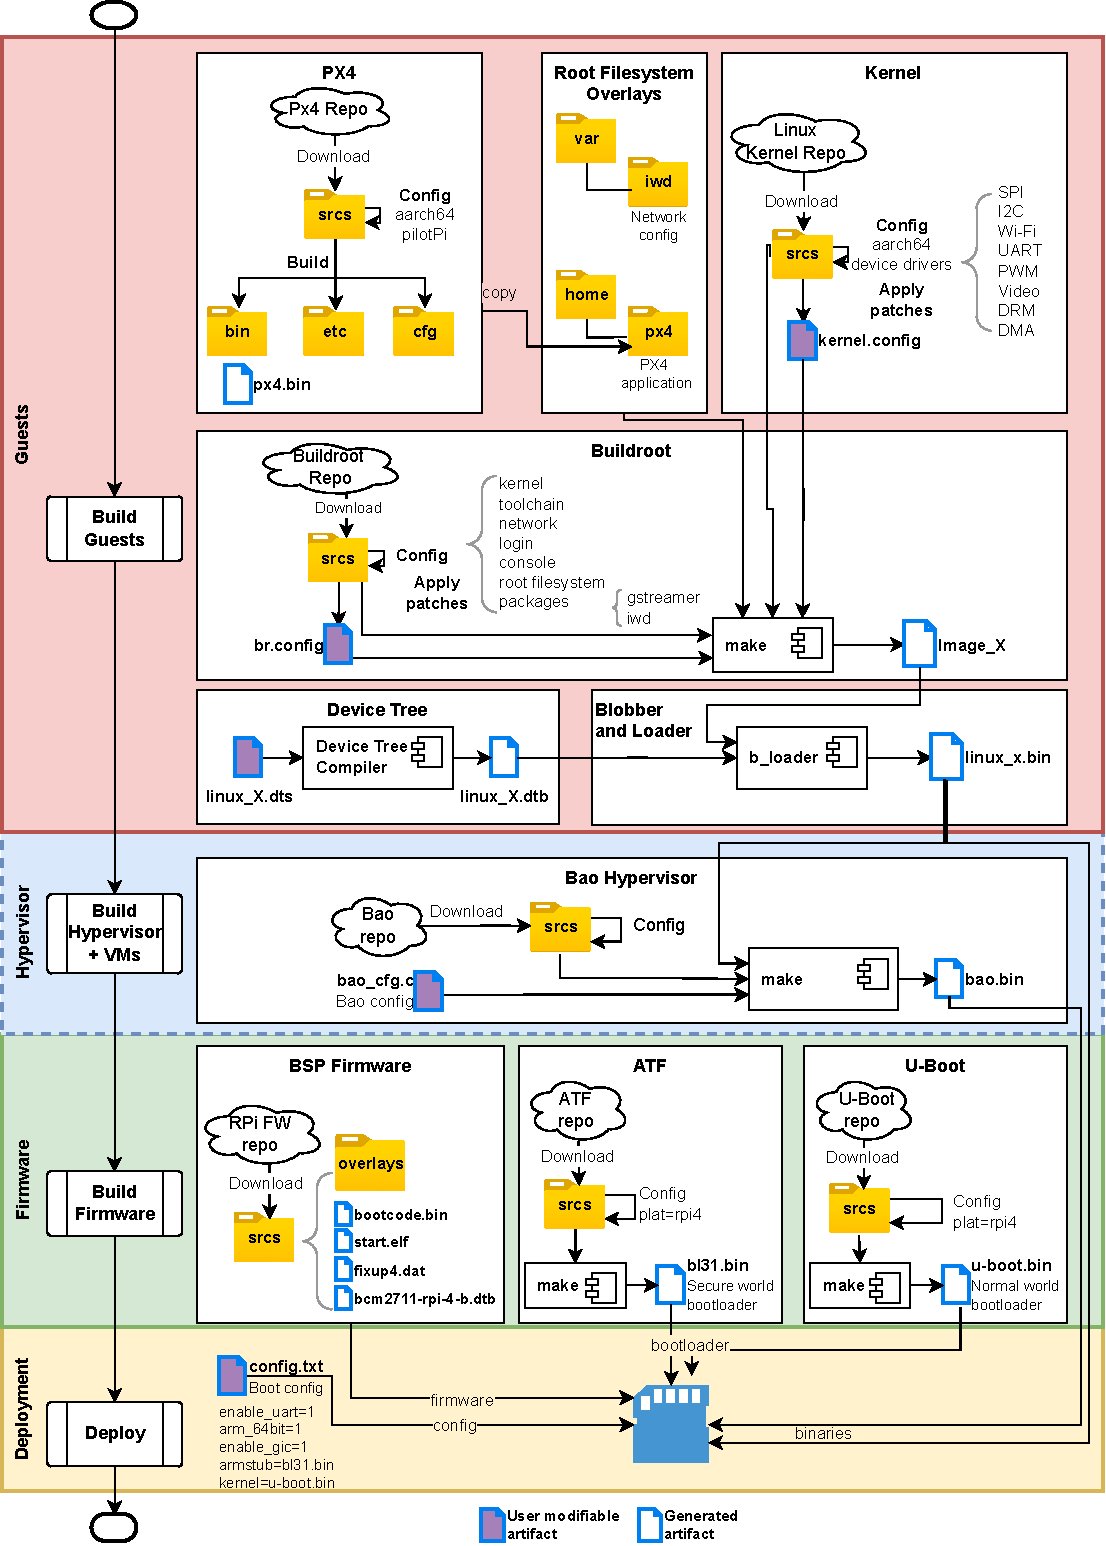
\includegraphics[width=1.0\textwidth]{./img/pdf/uav-main-Implem-Workflow} 
  \caption{Implementation workflow}%
  \label{fig:uav-main-Implem-Workflow}
\end{figure}

The first step is to build the guests. Only one ``guest'' can run natively at a
time in the \gls{uspfs} scenario, with
PX4 and video surveillance features encompassed in a single binary. On the other
hand, PX4 and video surveillance guests execute simultaneously and in isolation
in the \gls{sspfs} scenario. Thus, we start by building the PX4 application to
run on the \texttt{PilotPi} board with the \texttt{aarch64} architecture,
yielding a set of binaries and configuration files that can be deployed to the
\gls{uavic} platform. Then, we copy these files to a special directory --- the
Root Filesystem Overlays --- alongside with the network configuration to be
deployed by the selected embedded Linux build system (Buildroot) when compiling
the guest binary.
Next, we configure the Linux kernel to add support for the required device
drivers, such as \gls{spi}, \gls{i2c}, Wi-Fi, video, among others. We then
configure the embedded system to include the preconfigured kernel and to deploy
the PX4 application to the target, alongside with the network, login, console
and packages (e.g., \texttt{gstreamer} for video and \texttt{iwd} for wireless
network setup). Buildroot compiles a Linux image \texttt{Image\_X}, where
\texttt{X} is the guest's number. Next, we configure the device tree source \texttt{linux\_X.dts} to
match the available hardware for each guest and compile it to generate a \gls{dtb} \texttt{linux\_X.dtb}. The \gls{dtb} is then wrapped together
with the Linux's guest image \texttt{Image\_X} by the \texttt{b\_loader}
component, yielding an executable that can be deployed to the \gls{uavic}
platform with minimal dependencies and matching the required hardware. In the
\gls{uspfs} case we have an unique binary to deploy; in the \gls{sspfs} case,
however, we need to repeat the process for each guest to comply with the
requirements, yielding two binaries which will later on be merged by the Bao
hypervisor when generating the target's executable.

Secondly, and only for the \gls{sspfs} case, we create a configuration for the
Bao's hypervisor (\texttt{bao\_cfg.c}) describing each guest's build path
and entry point, the number 
of \glspl{cpu}, the memory regions, and the devices' memory and interrupts the
interrupts. This configuration file is used to setup each guest in the Bao
hypervisor and then merged them to generate a unique blob (\texttt{bao.bin}) containing the two guests atop of the hypervisor.

Next, we build the platform's firmware. We download the \gls{bsp} firmware for
the Raspberry Pi 4, containing the board's firmware, the first stage bootloader
and the device tree blob to boot the board. We configure and build the
\gls{atf} (\texttt{bl31.bin}), required by the Bao hypervisor. Then, we
configure and build the normal world bootloader (\texttt{u-boot.bin}), which
will be used to load the target binary --- \texttt{linux\_x.bin} in the
\gls{uspfs} case or \texttt{bao.bin} in the \gls{sspfs} case.

Lastly, we deploy the boot artifacts to the \gls{sd} card, containing the
Raspberry Pi 4 firmware, the secondary bootloaders, the target binary
(\texttt{linux\_x.bin} or \texttt{bao.bin}) and a configuration file
(\texttt{config.txt}). The configuration file sets up the boot process, enabling
the \gls{uart} and \gls{gic} subsystems, and pointing to the secondary
bootloaders which will be invoked after the initial board boot up is completed.

For further clarification of the deployment stage, it is important to analyze
the \gls{uavic} boot flow, depicted in Fig.~\ref{fig:uav-main-rpi4-boot}. The
first stage bootloader (\texttt{bootcode.bin}) initializes the hardware, loads
the firmware from the \gls{sd} card and reads the \texttt{config.txt} file to
parse the boot parameters.

\begin{figure}[!hbt]
  \centering
  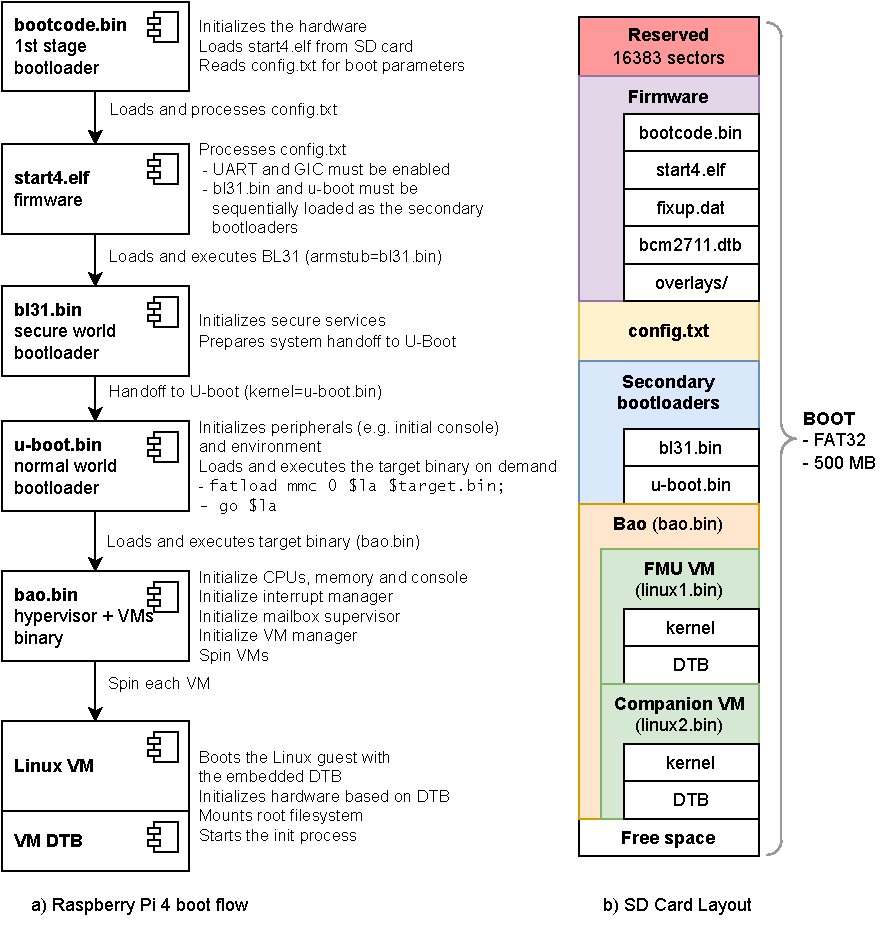
\includegraphics[width=0.9\textwidth]{./img/pdf/uav-main-rpi4-boot} 
  \caption{UAVIC boot: a) platform boot flow; b) SD card layout}%
  \label{fig:uav-main-rpi4-boot}
\end{figure}

The firmware (\texttt{start4.elf}) processes \texttt{config.txt}, which in this case,
means it must enable \gls{uart} and \gls{gic} and that the secondary bootloaders
--- \texttt{bl31.bin} and \texttt{u-boot.bin} ---
must be sequentially loaded. 
%
It then loads and executes \texttt{bl31.bin} which initializes the secure
services and prepares system handoff to the normal world bootloader
\texttt{u-boot.bin}.
%
Next, control is handed to \texttt{u-boot.bin}, which initializes the peripherals
(e.g. initial console) based on the firmware's \gls{dtb} and the
environment. \texttt{u-boot.bin} allows to load and execute the target binary on
demand, whether through boot parameters stored in a U-Boot script or directly in the console.

The target binary is then executed: \texttt{linux\_x.bin} for the \gls{uspfs}
case or \texttt{bao.bin} for the \gls{sspfs} case. We will focus on the latter,
which is a superset of the former. The Bao hypervisor initializes the
\glspl{cpu}, memory and system console, the interrupt manager, the mailbox
supervisor, and, lastly, the \gls{vm} manager. After completing the
initialization it spins each \gls{vm} which boots the Linux guest with the
embedded \gls{dtb}, initializes the hardware based on the guest's configuration
file and the \gls{dtb}, mounts the root filesystem and starts the \texttt{init}
process. Each guest is now executing in isolation, supervised by the Bao
hypervisor.

\section{Base system}
\label{sec:base-system}
The base system represents the common set of hardware and software components
required for the implementation of the \gls{uspfs} and the \gls{sspfs}
solutions. It comprises the \gls{uav}'s assembly and configuration, and the testing and
validation of the PX4 and video surveillance stacks.

\subsection{UAV assembly}
\label{sec:uav-assembly}
The first step is to assemble the \gls{uav} and configure it using the \gls{gcs}
running on the ground station. Fig.~\ref{fig:uav-assembly} displays the
assembled \gls{uav}, based on the HoverGames kit, on the left, and the QGroundControl software (\gls{gcs})
used to configure it. 

\begin{figure}[!hbt]
  \centering
  \includegraphics[width=0.8\textwidth]{./img/png/uav-assembly-annot-final} 
  \caption[UAV assembly and configuration]{UAV assembly and configuration: UAV
    (left); Ground Station running QGroundControl (right)}%
  \label{fig:uav-assembly}
\end{figure}

The S500 frame (3) forms the base for assembling the drone, including the
landing gear, the arms, and the support plates for the electronics.
The \gls{gps} NEO-M8N module (1), included in the HoverGames kit, was installed due to its
cost-effectiveness and accuracy even in scenarios where urban canyon or weak
signals are involved~\cite{gps-neom8n-product}. The four brushless \gls{dc}
motors (2) were installed on the outer extremities of the arms, controlled by
\glspl{esc} 40 Ampere optocoupled devices. 

A \gls{lipo} battery (12) with 3 cells series configuration (3S) was selected,
with a 5000 mAh capacity and with a matching XT-60 connector
(4)~\cite{lipo-3s-uav}, yielding an expected flight autonomy of about 30 minutes in full throttle. PilotPi was assembled on top of the Raspberry Pi 4
to form the \gls{uavic} platform (7). The \gls{gcs} running QGroundControl (11)
communicates with the \gls{uav} using the telemetry radio link (5)(6). An
optional \gls{uart} port (8) was added to the \gls{gcs} to debug the
\gls{uavic}'s boot process, which is excluded from the final
implementation. Lastly, the two \gls{usb} devices required by the video
surveillance application --- Wi-Fi dongle (9) and camera (10) --- were installed
in the \gls{uavic}.

To configure the \gls{uav} the User must power on the \gls{uavic} and start the
PX4 flight stack, which communicates with QGroundControl through the telemetry
radio or Wi-Fi to setup the device. Thus, first, we must deploy PX4 to the
\gls{uavic}.

\subsection{PX4}
\label{sec:px4}
Next, to validate the assembly we initially deployed PX4 to the \gls{uavic}
platform directly on top of a general purpose Linux
\gls{os}. Listing~\ref{lst:build-pilotpi} presents the PX4's build script: (1)
the autopilot sources are downloaded and the submodules for the NuttX
applications running as tasks in PX4 are recursively updated; (2) a Python
virtual environment is created and activated to support the build; (3) PX4 is
built for the PilotPi platform with the Arm 64-bit architecture; (4) we setup
the autopilot host \gls{ip} address and username to upload PX4 to the
\gls{uavic} and to backup the files to the local buildroot folder.

\begin{longlisting}
\centering
\inputminted[]{bash}{./listing/buildPilotPi.sh}
\caption{PX4 build script}
\label{lst:build-pilotpi}
\end{longlisting}

To configure PX4 we use the \texttt{kconfig} configuration system adopted by the
NuttX \gls{rtos}. Listing~\ref{lst:cfg-pilotpi} shows an excerpt of the
configuration file where we setup the platform and architecture, the toolchain,
and the required drivers and modules.

\begin{longlisting}
\centering
\inputminted[]{kconfig}{./listing/px4.config}
\caption{PX4 configuration file (excerpt)}
\label{lst:cfg-pilotpi}
\end{longlisting}

PX4 relies on a boot script to configure the \gls{uav} and to enable the modules,
services, and communications to be used by the
aircraft. Listing~\ref{lst:pilotpi-mc} presents the startup script --- \texttt{pilotpi\_mc.config} ---
which: (1) imports the \gls{uav}'s saved parameters; (2) sets up the vehicle
type and airframe;  (3) configures the camera to be triggered via Mavlink
protocol; (4) starts the management services for mission and
geofence data, \gls{cpu} load monitoring, and battery status monitoring; (5) initializes all sensors and actuators; (6) initializes the
\gls{rc} management task; (7) starts the main state machine of the \gls{fmu}; 
(8) starts all the multicopter's tasks, such as, navigation, position, attitude
and rate control, and logging service, among others;
(9) enables Mavlink communications via telemetry radio and Wi-Fi; 
(10) signals boot is complete to the \gls{gcs}, allowing for
the User's configuration to start.

\begin{longlisting}
\centering
\inputminted[]{bash}{./listing/pilotpi-mc.config}
\caption{PX4 boot script}
\label{lst:pilotpi-mc}
\end{longlisting}

After uploading the PX4 application to the \gls{uavic} platform, we can execute
it as follows: \lstinline{./px4 -s pilotpi_mc.config}. Fig.~\ref{fig:uav-cfg-px4-boot} illustrates the PX4
execution. It can be observed that all sensors and actuators are successfully
initialized and that the Mavlink communications are started, more specifically,
the Wi-Fi link, which enables the \gls{gcs} to connect to it 
(\lstinline{partner IP: 192.168.1.37}).
  
\begin{figure}[!hbt]
  \centering
  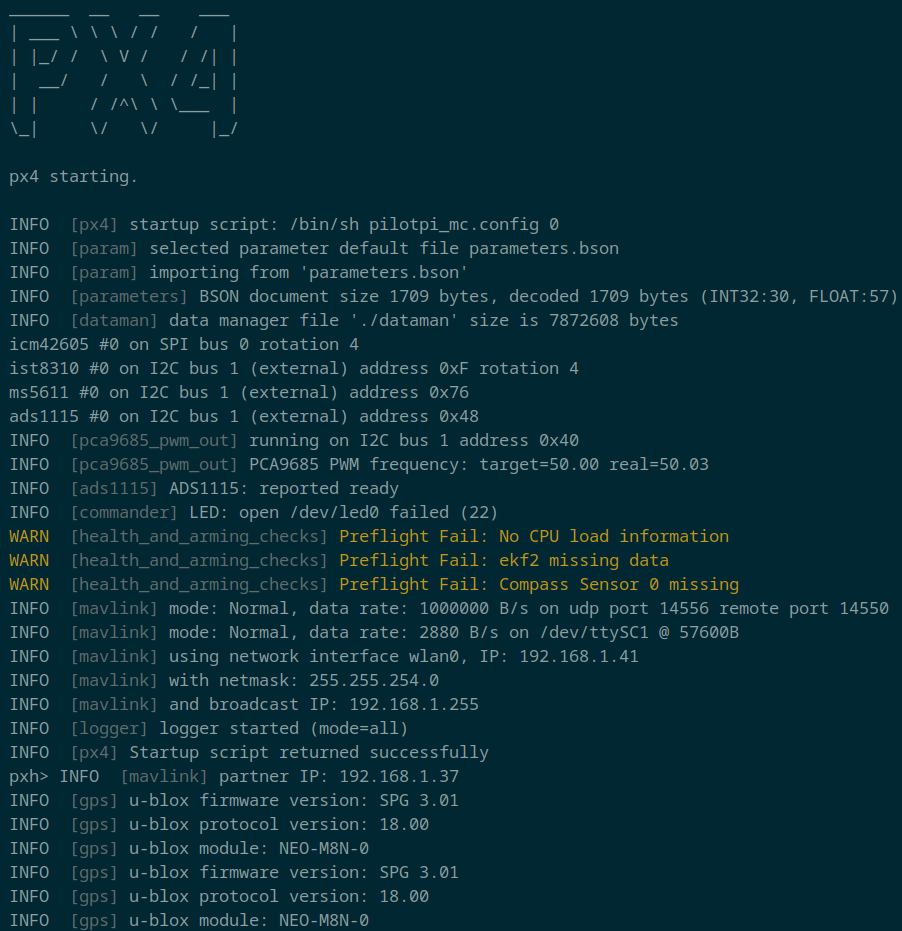
\includegraphics[width=0.6\textwidth]{./img/png/px4-boot} 
  \caption{UAV configuration: PX4 boot}
  \label{fig:uav-cfg-px4-boot}
\end{figure}

\subsection{UAV configuration}
\label{sec:uav-configuration}
After pairing the \gls{uav} to the \gls{gcs}, the User can configure the
aircraft. The User starts by defining the airframe to a quadrotor X type, more
specifically, the NXP HoverGames (see Fig.~\ref{fig:uav-cfg-airframe}).

\begin{figure}[!hbt]
  \centering
  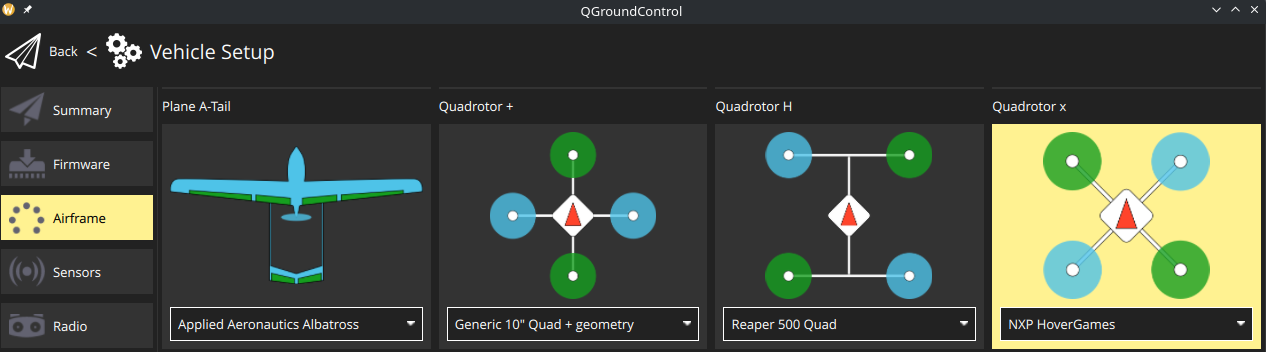
\includegraphics[width=0.9\textwidth]{./img/png/qgc-airframe} 
  \caption{UAV configuration: airframe}
  \label{fig:uav-cfg-airframe}
\end{figure}

Next, the User needs to calibrate the \gls{uav}'s sensors (see
Fig.~\ref{fig:uav-cfg-sensors}), namely the compass, the gyroscope and the
accelerometer by manipulating the \gls{uav} with the required motions.

\begin{figure}[!hbt]
  \centering
  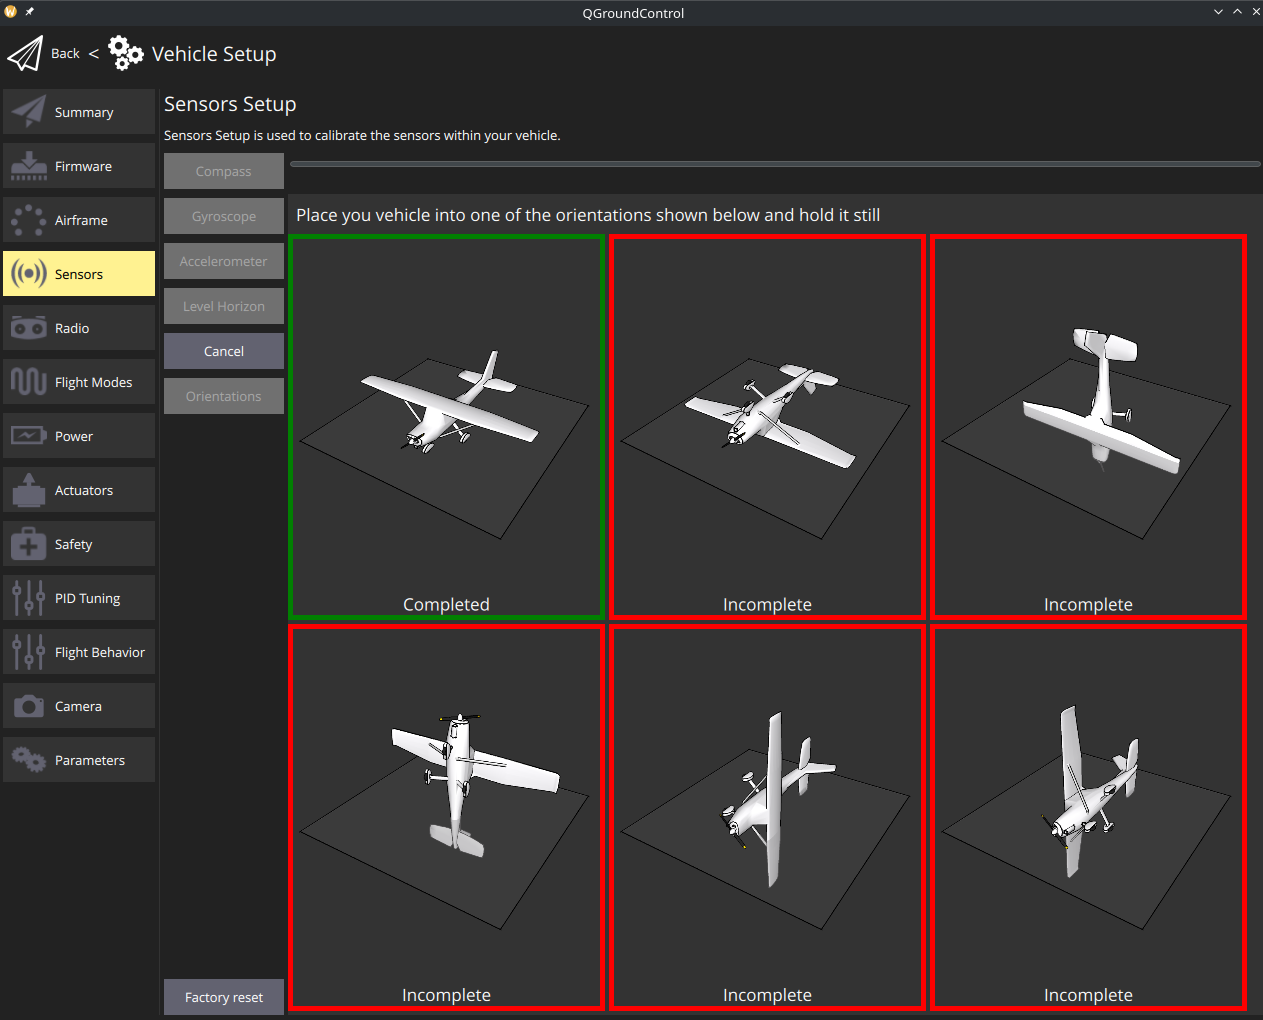
\includegraphics[width=0.8\textwidth]{./img/png/qgc-sensors} 
  \caption{UAV configuration: sensors' calibration}
  \label{fig:uav-cfg-sensors}
\end{figure}

Then, the User configures the power management (see
Fig.~\ref{fig:uav-cfg-power}) by setting up the source, the number of cells and
calculating the voltage divider. Additionally, the User must also calibrate the
\gls{esc} \gls{pwm} minimum and maximum values to avoid outputs' saturation.

\begin{figure}[!hbt]
  \centering
  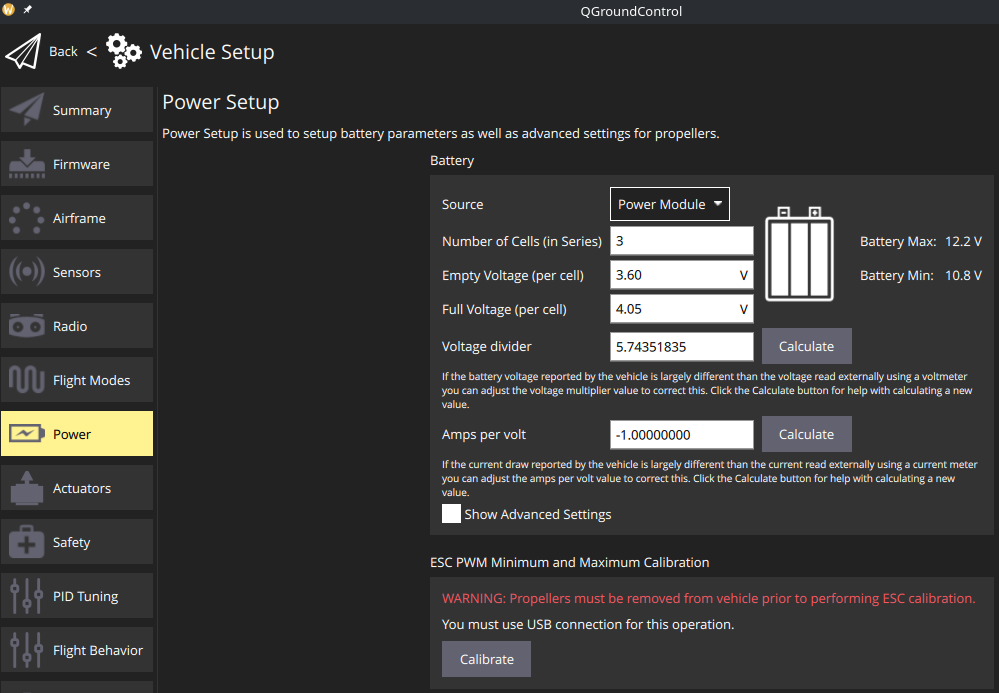
\includegraphics[width=0.8\textwidth]{./img/png/qgc-power} 
  \caption{UAV configuration: power management}
  \label{fig:uav-cfg-power}
\end{figure}

After configuring the power, the User needs to calibrate the actuators (see
Fig.~\ref{fig:uav-cfg-actuators}) defining the number of motors and its
geometry (position and direction) and assigning each motor to an output
channel. Then, and after removing the propellers, the User must test the motors
to validate the calibration, e.g., verifying that each motor rotates accordingly
to the picture presented and that the velocity varies with the slider.

\begin{figure}[!hbt]
  \centering
  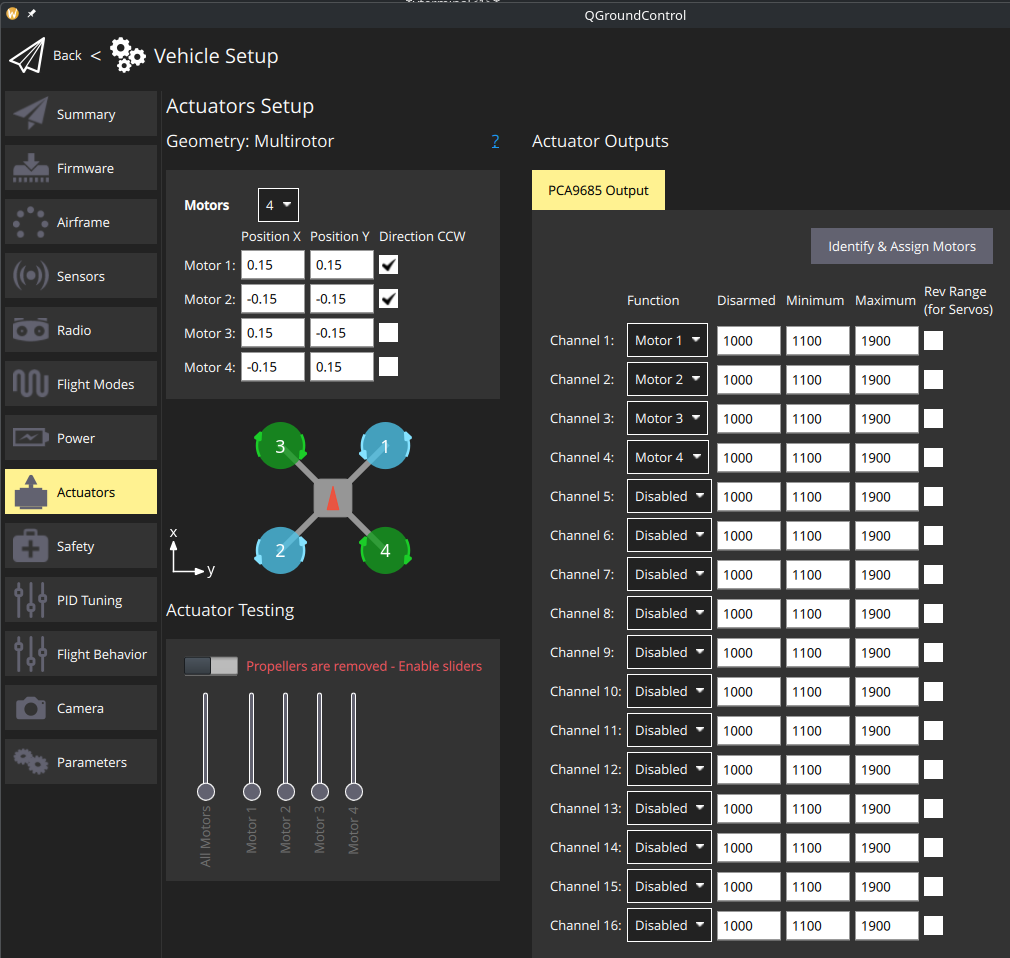
\includegraphics[width=0.75\textwidth]{./img/png/qgc-actuators} 
  \caption{UAV configuration: actuators}
  \label{fig:uav-cfg-actuators}
\end{figure}


Fig.~\ref{fig:uav-cfg-summary} presents the \gls{uav}'s setup summary,
demonstrating that the configuration was correctly performed. Then, the User can
copy the parameters' database from the current PX4 deployment to any number of
PX4 instances, as long as the \gls{uav} characteristics remain the same.

\begin{figure}[!hbt]
  \centering
  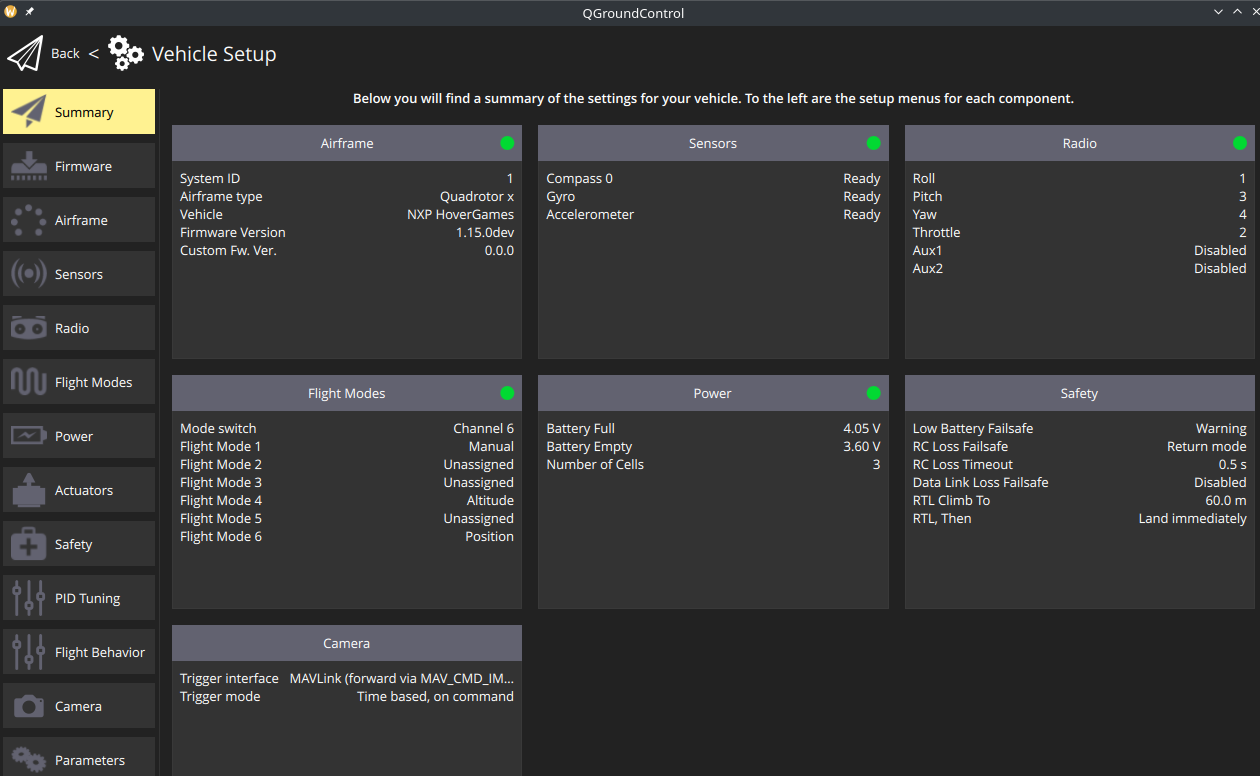
\includegraphics[width=0.9\textwidth]{./img/png/qgc-summary} 
  \caption{UAV configuration: summary}
  \label{fig:uav-cfg-summary}
\end{figure}

\subsection{Video surveillance}
\label{sec:video-surveillance}

Next, we implemented and validated the video surveillance pipeline --- presented
in the design stage and illustrated in Fig.~\ref{fig:uav-design-unsup} --- using the
\texttt{gstreamer} multimedia framework due to its open-source multi-platform
nature, modular architecture supporting a wide range of video codecs,
support for video streaming over a network, and easy setup of the video
pipeline. These features were crucial for the fast iteration and simplified testing
of the implementation.

The video surveillance sender, running in the \gls{uav}, is responsible for
grabbing the frames with an adequate resolution and framerate in the MJPEG
format, decode each frame and encode with the H.264 codec which is then packed
in the \gls{rtsp} to be sent by \gls{udp}. Listing~\ref{lst:gstreamer-sender}
shows the shell script used to test the video surveillance sender's pipeline. We
specify the \texttt{device} to match the \gls{usb} camera with a resolution of
640 x 480 pixels and a framerate of 30 \gls{fps}, and the host \gls{ip} address
and port to ensure that only the \gls{gcs} can receive the video frames.

%\hfill \break% 
%\hfill \break% 

\begin{longlisting}
\centering
\inputminted[]{bash}{./listing/gstreamerSender.sh}
\caption{Video surveillance sender script}
\label{lst:gstreamer-sender}
\end{longlisting}

Conversely, the video surveillance receiver, running in the \gls{uav}, must
connect to an \gls{udp} port, decode and unpack the \gls{rtsp} stream, convert
it to a suitable format and render it on screen for the \texttt{User}.
Listing~\ref{lst:gstreamer-receiver}
shows the shell script used to test the video surveillance receiver's
pipeline. We specify the \gls{udp} \texttt{port} to match the sender, the H.264
video codec to decode the video stream, and the \texttt{autovideosink} to
display the video on the screen.

%\hfill \break% 
%\hfill \break% 
\begin{longlisting}
\centering
\inputminted[]{bash}{./listing/gstreamerReceiver.sh}
\caption{Video surveillance receiver script}
\label{lst:gstreamer-receiver}
\end{longlisting}


Fig.~\ref{fig:px4-qgc-cam} demonstrates the video surveillance pipeline
validation. In this test case, the PX4 (Fig.~\ref{fig:px4-qgc-cam-2}) and the video
surveillance sender (Fig.~\ref{fig:px4-qgc-cam-3} -- top) run
simultaneously on top of a generic Linux OS in the \gls{uavic}. Then, on the \gls{gcs}, we start
the video pipeline receiver (Fig.~\ref{fig:px4-qgc-cam-3} -- bottom) and
QGroundControl. We can observe in Fig.~\ref{fig:px4-qgc-cam-1} that PX4 and video
surveillance applications are simultaneously running on the \gls{uavic},
successfully displaying the \gls{uav} information in QGroundControl and the video stream in \texttt{gstreamer}.

\begin{figure}[htb!]
  \centering
  %
  \begin{subfigure}[t]{.48\textwidth}
    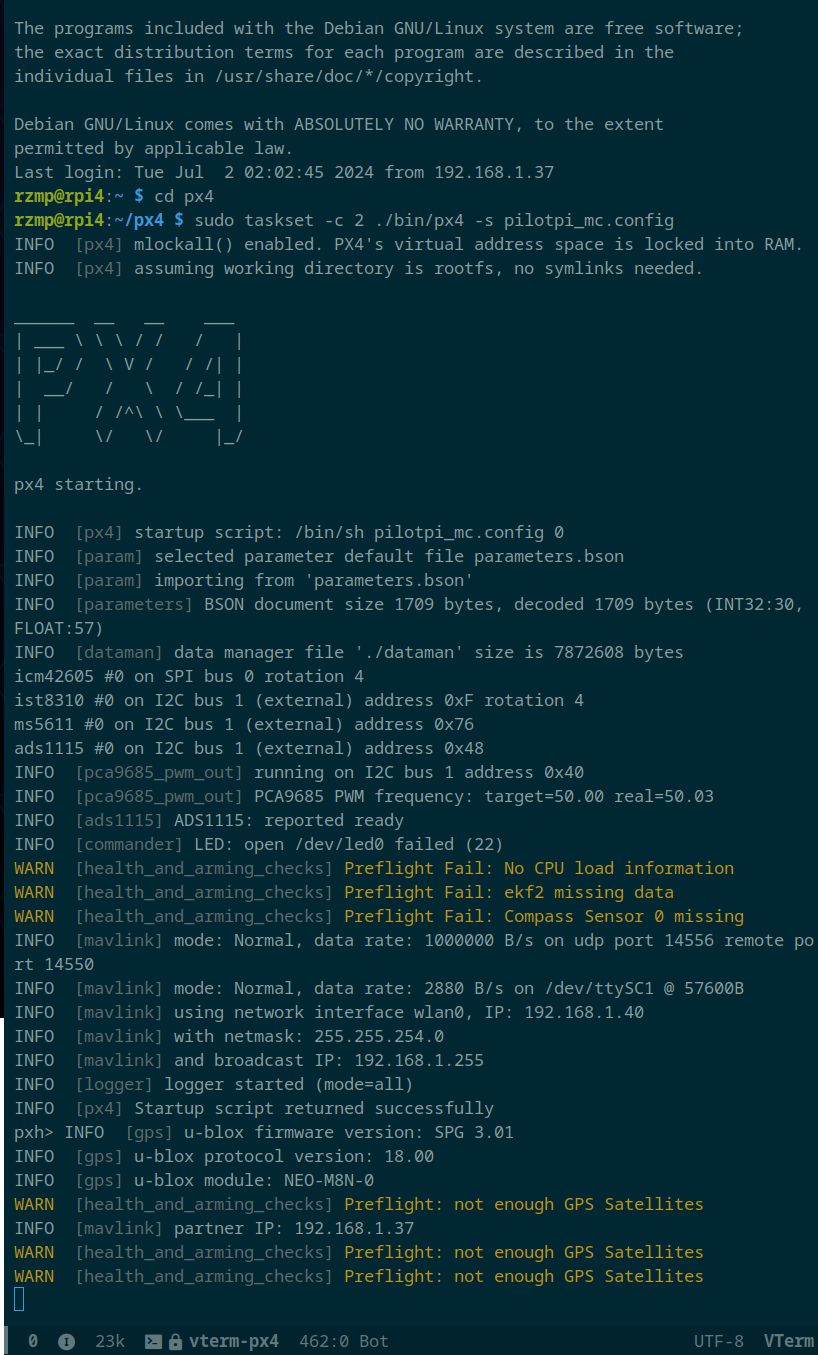
\includegraphics[width=0.89\textwidth]{./img/png/px4-qgc-cam-2}
  \caption{PX4 boot}%
  \label{fig:px4-qgc-cam-2}
  \end{subfigure}
%
  \begin{subfigure}[t]{.48\textwidth}
    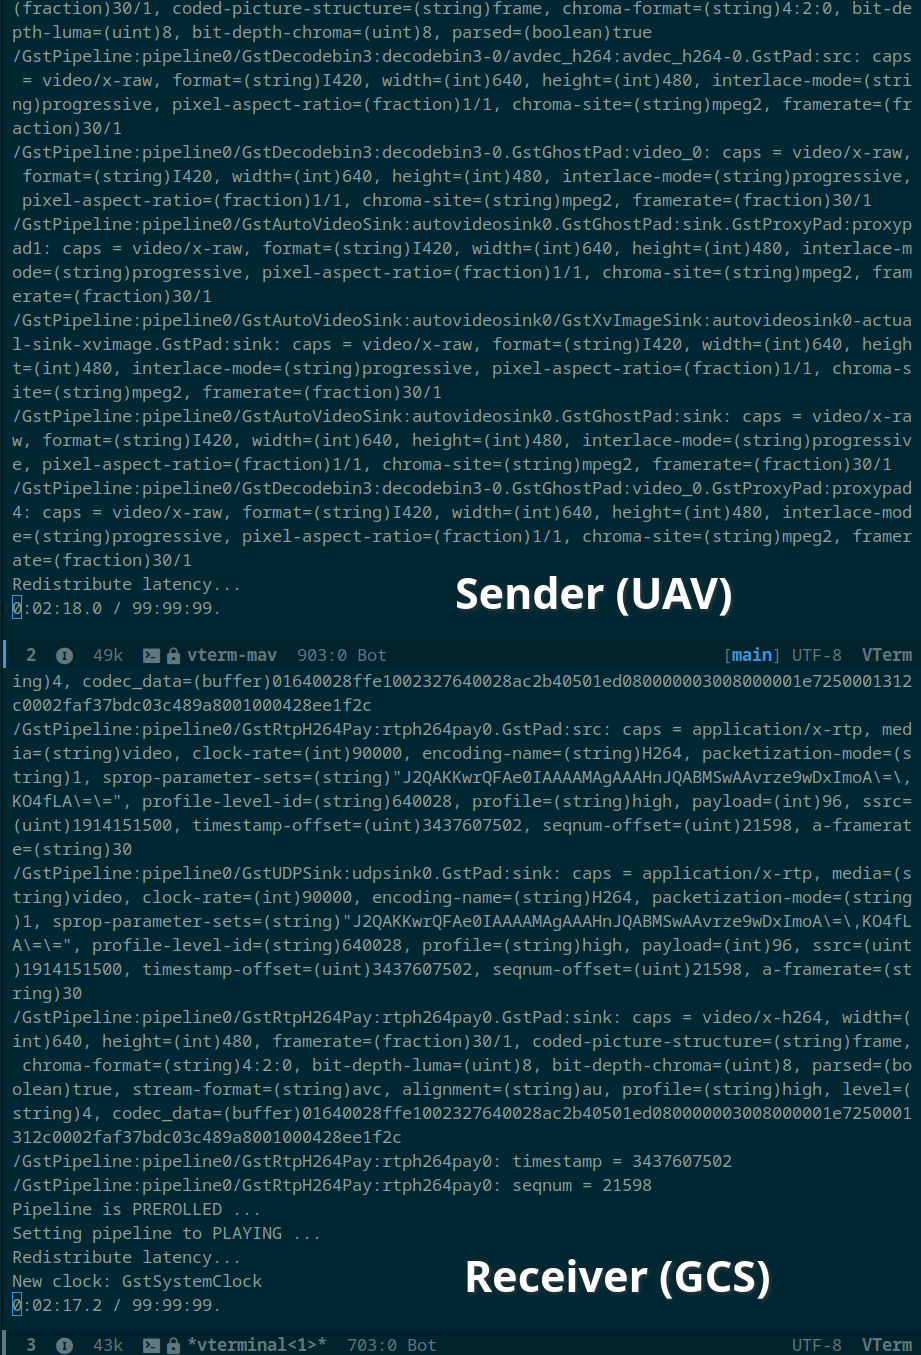
\includegraphics[width=1.0\textwidth]{./img/png/px4-qgc-cam-3}
  \caption{Video pipeline: sender (UAV); receiver (GCS)}%
  \label{fig:px4-qgc-cam-3}
  \end{subfigure}
%
  \begin{subfigure}[t]{.48\textwidth}
    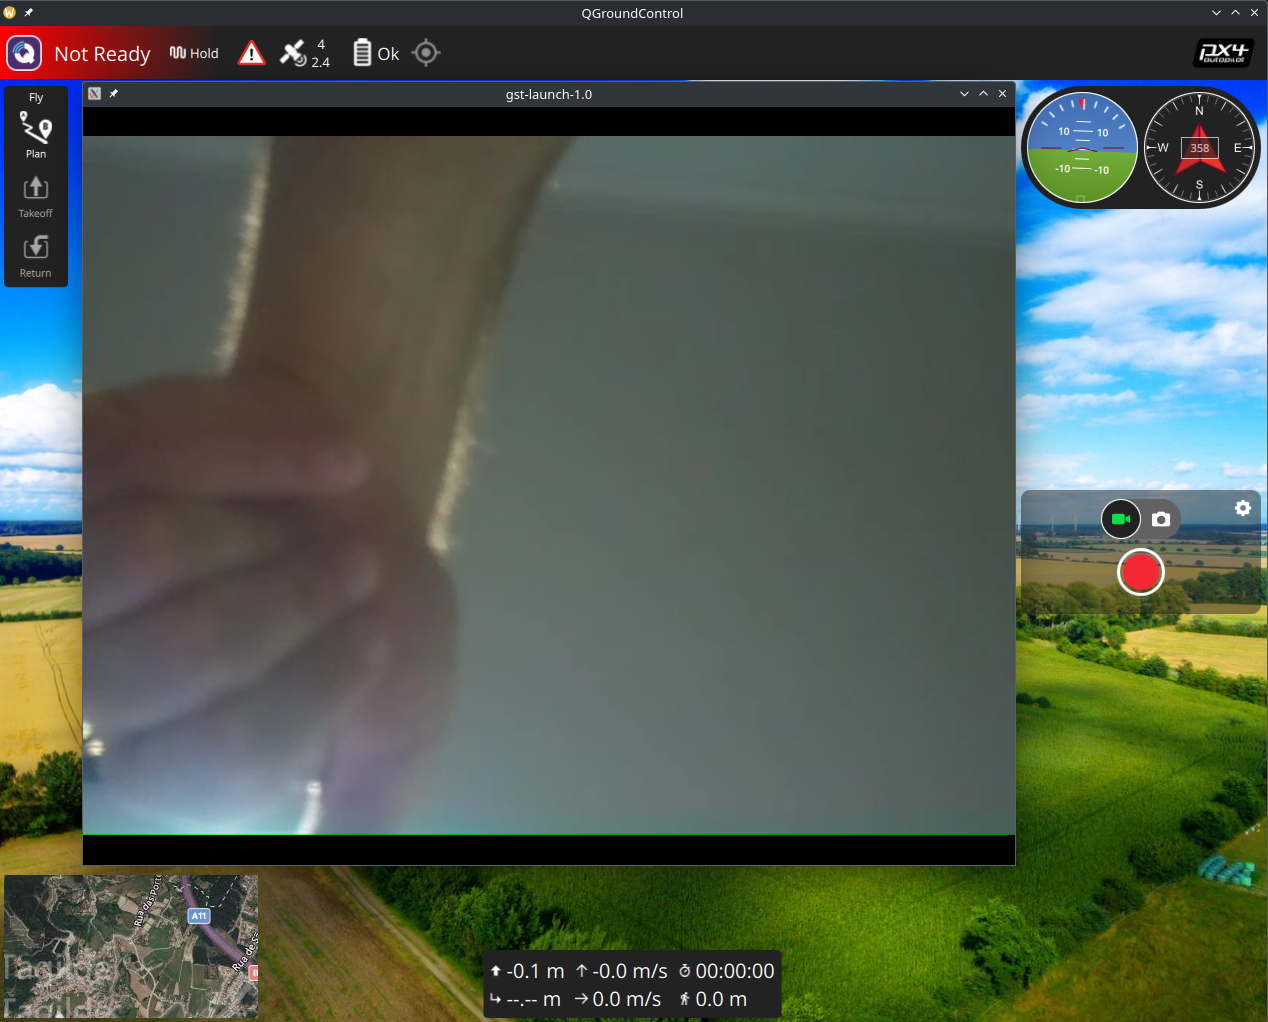
\includegraphics[width=1.0\textwidth]{./img/png/px4-qgc-cam-1}
  \caption{QGroundControl and video surveillance receiver}%
  \label{fig:px4-qgc-cam-1}
  \end{subfigure}
  % 
  \caption{Video surveillance pipeline validation}%
  \label{fig:px4-qgc-cam}
\end{figure}

\section{USPFS}
\label{sec:uspfs-implem}
The \gls{uspfs} solution aggregates PX4 and the video surveillance pipeline
running in the \gls{uavic} on top of a custom embedded Linux-based
\gls{os}. The kernel configuration must add support for the device drivers
required for both software stacks. We've selected the latest stable release of
the \href{https://github.com/raspberrypi/linux}{Linux kernel for the Raspberry Pi's platform} (version
6.6). Listing~\ref{lst:kernel-uspfs} shows the kernel configuration for the
\gls{uspfs} solution comprising: PX4 -- \gls{spi} and \gls{i2c} for the sensors
and actuators, \gls{pwm} for the motors, PL011 for the \gls{rc} \gls{uart}; video
surveillance -- video device drivers and modules and the \lstinline{MT7921U}
module for the Mediatek \gls{usb} Wi-Fi dongle.

\begin{longlisting}
\centering
\inputminted[]{kconfig}{./listing/kernel-uspfs.config}
\caption{USPFS: kernel configuration file (excerpt)}
\label{lst:kernel-uspfs}
\end{longlisting}

Then, we configured Buildroot (see Listing~\ref{lst:br-uspfs}): (1) to use the
preconfigured kernel; (2) setup the root filesystem and its overlay to include
the previously built PX4; (3) setup the boot debug console to UART5
(\texttt{ttyAMA5}); (4) add Busybox to bootstrap the most important \gls{os}
utilities; (5) add the \texttt{GStreamer} package for video surveillance; (6)
add support for the \gls{usb} Wi-Fi dongle. The custom Linux \gls{os} is
built, yielding an \gls{os} image -- \texttt{Image\_1}.

\begin{longlisting}
\centering
\inputminted[]{kconfig}{./listing/br-uspfs.config}
\caption{USPFS: buildroot configuration file (excerpt)}
\label{lst:br-uspfs}
\end{longlisting}

Next, we customized the Linux device tree to include all the necessary hardware
for the \gls{uspfs} solution, as previously illustrated in
Fig.~\ref{fig:hw-map-1}. The Linux \gls{os} image and the device tree are used
to generate an executable -- \texttt{linux\_1.bin} -- that is able to run on the
\gls{uavic} platform.

The next step was to build the firmware. We downloaded the \gls{bsp} firmware
for the Raspberry Pi 4, and configured and built the secondary bootloaders --
\texttt{bl31.bin} and \texttt{u-boot.bin}. To inspect the boot process we used
the only available \gls{uart} port --- UART5 (\lstinline{ttyAMA5}) --- which
differs from the default one used by \texttt{bl31.bin} (UART0). Thus, the
\gls{atf} source code needed to be patched to accomodate for this
change (see Listing~\ref{lst:atf-patch}). We replace \lstinline{serial0} by
\lstinline{serial5} in the Raspberry Pi 4 \texttt{bl31} setup and modify the
\gls{uart} offset to point to UART5.

\begin{longlisting}
\centering
\inputminted[]{makefile}{./listing/atf-patch.mk}
\caption{USPFS: ATF patch}
\label{lst:atf-patch}
\end{longlisting}

U-Boot does not require patching, as it inherits the modified device tree used
by \texttt{bl31.bin}. Listing~\ref{lst:uboot-mk} shows the U-Boot makefile. We
download the latest stable release (\lstinline{v2024.07}) and use the Raspberry
Pi 4 default \texttt{config} to configure it. Then, we modify the U-Boot
environment to automatically boot the \gls{uavic} when powering and build it. On startup,
U-Boot will evaluate the \texttt{bootcmd} command which loads the binary to the
defined address \lstinline{0x80000}, immediately after the
\texttt{bl31.bin}.

\begin{longlisting}
\centering
\inputminted[]{makefile}{./listing/uboot.mk}
\caption{USPFS: U-Boot makefile}
\label{lst:uboot-mk}
\end{longlisting}

Lastly, we deploy the custom Linux image (\texttt{linux\_1.bin}) to the SD card,
alongside with the Raspberry Pi firmware, the secondary bootloaders
(\texttt{bl31.bin} and \texttt{u-boot.bin}), and the boot configuration file for
the platform --- \texttt{config.txt}. Listing~\ref{lst:uspfs-cfg-txt} displays
the \texttt{config.txt} file, where we enable the \gls{gic} subsystem to handle
early interrupts (e.g., associated to the console), we define the secondary
bootloaders, and we setup the firmware's console -- which might be required
for early debug of the boot process.

\begin{longlisting}
\centering
\inputminted[]{kconfig}{./listing/config.txt}
\caption{USPFS: Deployment -- config.txt}
\label{lst:uspfs-cfg-txt}
\end{longlisting}

Then, we inserted the SD card in the \gls{uavic} and powered on the platform,
connecting the \gls{uart} debug cable in the host computer to inspect the boot
process using a terminal emulator with serial communication capabilities to open
a serial port with a baudrate of 115200 bits/second: 
\lstinline{screen /dev/ttyUSB0 115200}. 
Listing~\ref{lst:uspfs-boot} shows the \gls{uspfs}'s boot log, where we can
identify the versions of
the Linux kernel and the Buildroot's toolchain, and the setup of the early
console to UART5. 

\begin{longlisting}
\centering
\inputminted[]{kconfig}{./listing/boot-uspfs.txt}
\caption{USPFS: Boot log (excerpt)}
\label{lst:uspfs-boot}
\end{longlisting}

Finally, we tested the PX4 and video surveillance
applications, applying the same procedure as described in Sections~\ref{sec:px4}
and~\ref{sec:video-surveillance}. Both applications executed correctly in the
\gls{uspfs} system, validating the implementation.

\section{SSPFS}
\label{sec:sspfs-implem}
In the \gls{sspfs} solution, the goal is to build two separate
Linux \glspl{os} -- here called \textbf{guests} -- one for the PX4 stack, and
another one for the video surveillance one, that run atop of the Bao
hypervisor. The process of building a guest is similar to the one shown for the
\gls{uspfs} solution, but duplicated. For each guest: (1) we selected the
required kernel drivers and packages, and compiled a Linux \gls{os} image --
\texttt{Image\_X}; (2) we customized a Linux \gls{dts} and used it alongside \texttt{Image\_X} to generate an executable Linux \gls{os}
binary \texttt{linux\_x.bin}. Thus, at end of this stage, we have two binaries
named \texttt{linux\_1.bin} (PX4) and \texttt{linux\_2.bin} (video surveillance). 

The next step is to \textbf{build the hypervisor and the \glspl{vm}}. We
\href{https://github.com/ElectroQuanta/bao-hypervisor-porting}{forked the Bao
  hypervisor repository} and cloned it locally. Again, to inspect the Bao's boot
process it is best to have UART5 as the Bao's default console
for the platform, as opposed to UART0. Thus, we needed to patch Bao to support
this. Bao relies on a platform description file (see Listing~\ref{lst:rpi4-desc}) to assess the platform's capabilities, namely:
the \gls{cpu} number, the memory regions, the console's base address, and the
\gls{gic} description. Line 15 shows the console's base address --- changed to
\lstinline{0xfe201000} --- which must be aligned to a 4 KB memory page. Then, in
the platform's header file (see Listing~\ref{lst:rpi4-plat-header}) we configured
the \gls{uart}'s clock to 48 MHz and the console's address offset to
\lstinline{0xa00}, yielding UART5's address (\lstinline{0xfe201a00}).

\begin{longlisting}
\centering
\inputminted[]{c}{./listing/rpi4_desc.c}
\caption{SSPFS: Bao's Raspberry Pi 4 platform description patch}
\label{lst:rpi4-desc}
\end{longlisting}

\begin{longlisting}
\centering
\inputminted[]{c}{./listing/platform.h}
\caption{SSPFS: Bao's Raspberry Pi 4 platform header patch}
\label{lst:rpi4-plat-header}
\end{longlisting}

Then, we created a custom Bao's configuration for each guest to describe its
available resources (see Listing~\ref{lst:bao-sspfs-cfg}). Lines 1 and 2 show the
\lstinline{VM_IMAGE} image that associates each \gls{vm} image to its path on
the host's filesystem. Lines 5 -- 14 define the memory regions for each guest,
starting at \lstinline{0x0b400000}, immediately after the \texttt{bao.bin}
placement in memory. PX4's first memory region, with a size of 144 MB, was placed in the first 1 GB of
memory due to its requirements for \gls{dma} access, which is only available in
this memory slot. A second memory region of 3 GB was mapped for this \gls{vm},
even though not required, as the platform allows it. The video surveillance
\gls{vm} has two memory regions: the first one of 624 GB due to the heavy memory
requirements of the video pipeline; an extra optional region of 2 GB as the
platform allows it. Lines 15 and 16 define an extra memory region for the
\gls{pcie} bus, required by the \gls{usb} devices, namely the \gls{usb} camera.

For the PX4 \gls{vm} we assigned one \gls{cpu} core, the two memory regions and
nine devices as indicated in the design phase (revisit
Fig.~\ref{fig:hw-map-2}). For the video surveillance \gls{vm} we assigned the
remaining three \gls{cpu} cores, the two memory regions and four devices as
indicated in the design phase (revisit Fig.~\ref{fig:hw-map-3}). It is also
important to highlight the two repeated devices --- the architectural timer and
the mailbox. The first one is automatically handled by Bao; the second one was
now introduced to support the mailbox sharing across guests.

\begin{longlisting}
\centering
\inputminted[]{c}{./listing/bao-sspfs-cfg.c}
\caption{SSPFS: Bao's configuration}
\label{lst:bao-sspfs-cfg}
\end{longlisting}

The \textbf{mailbox supervision} implementation follows the design presented in
Fig.~\ref{fig:design-mailbox} and requires the addition of the
mailbox manager to the Bao hypervisor and the patch of the Linux kernel
mailbox driver for the Raspberry Pi firmware. Listing~\ref{lst:bao-mailbox-manager}
shows the mailbox manager added. Lines 1 -- 3 contain definitions for the
mailbox interrupt, and arguments signalling the start and the end of the
firmware's transaction. Line 5 initializes a \texttt{spinlock} -- a
synchronization primitive to ensure that only the current guest can access the
mailbox at a time. Lines 7 -- 9 setups the mailbox interrupt request handler,
which re-injects the interrupt into the current virtual \gls{cpu} in use and
then disables this interrupt source to prevent reentrance. Line 12--14 setups
the Raspberry Pi platform initialization routine which consists of assigning the
interrupt service routine to the interrupt management table to ensure it gets
activated when this interrupt is triggered. Lines 16--34 show the hypercall
callback: (1) when the transaction is started we lock the access to the mailbox
and enable its interrupt source to allow its supervised management; (2) when the
transaction ends we unlock the access to the mailbox and disable its interrupt
source, ending the supervised management by the current guest.

\begin{longlisting}
\centering
\inputminted[]{c}{./listing/rpi_firmware.c}
\caption{SSPFS: Mailbox manager added to Bao}
\label{lst:bao-mailbox-manager}
\end{longlisting}


Listing~\ref{lst:bao-init} shows Bao's initialization routine. Now, we added the
Raspberry Pi platform initialization, after interrupt management initialization
and before starting the \gls{vm} manager. This ensures we register the mailbox
supervisor only after interrupts are activated, and before executing the guests.

\begin{longlisting}
\centering
\inputminted[]{c}{./listing/init.c}
\caption{SSPFS: Bao initialization -- Raspberry Pi platform initialization}
\label{lst:bao-init}
\end{longlisting}

Listing~\ref{lst:bao-hypercall} shows the Raspberry Pi firmware mailbox
handling. Line 1 lists the hypercall sources, which now contain the mailbox
one. When the mailbox driver wants to start a transaction it triggers a
hypercall which is handled in the \lstinline{HC_RPI_FIRMWARE} case (line 15), invoking the
associated callback.

\begin{longlisting}
\centering
\inputminted[]{c}{./listing/hypercall.c}
\caption{SSPFS: Bao hypercall manager -- Raspberry Pi firmware mailbox handling}
\label{lst:bao-hypercall}
\end{longlisting}

Listing~\ref{lst:linux-rpi-fw} shows the patch performed on the Linux's mailbox
driver. Line 1 lists the hypercall sources, which now contain the mailbox
one. The relevant modifications are in lines 15 -- 21 and 42 -- 48. After
the driver locks the access to the mailbox, it will issue a hypercall, which
will be handled by Bao, signalling the transaction is starting. The mailbox
driver can now send a message to the mailbox, and upon completion or timeout,
another hypercall is issued to Bao, now signalling the transaction's end, after
which the driver releases the access to the mailbox.

\begin{longlisting}
\centering
\inputminted[]{c}{./listing/linux-rpi-fw.c}
\caption{SSPFS: Linux's Raspberry Pi mailbox driver -- patch}
\label{lst:linux-rpi-fw}
\end{longlisting}

Listing~\ref{lst:rpi-fw-validation-1} and Listing~\ref{lst:rpi-fw-validation-2} showcases the mailbox supervisor validation,
where both guests were executed atop of the Bao hypervisor. This allows to
assess the behavior of the system when both guests try to access the mailbox
\emph{simultaneously}. The PX4 \gls{vm} is remotely accessed using UART5, and the
video surveillance one using \texttt{ssh} over Wi-Fi. As can been seen, both
guests are able to successfully send transactions to the firmware's mailbox,
validating the implementation.

\begin{longlisting}
\centering
\inputminted[]{kconfig}{./listing/rpi-fw-validation-1.txt}
\caption{SSPFS: Mailbox supervisor validation -- PX4 VM boot log (excerpt)}
\label{lst:rpi-fw-validation-1}
\end{longlisting}

\begin{longlisting}
\centering
\inputminted[]{kconfig}{./listing/rpi-fw-validation-2.txt}
\caption{SSPFS: Mailbox supervisor validation -- Video VM boot log (excerpt)}
\label{lst:rpi-fw-validation-2}
\end{longlisting}


% \begin{figure}[htb!]
%   \centering
%   %
%   \begin{subfigure}[t]{.64\textwidth}
%     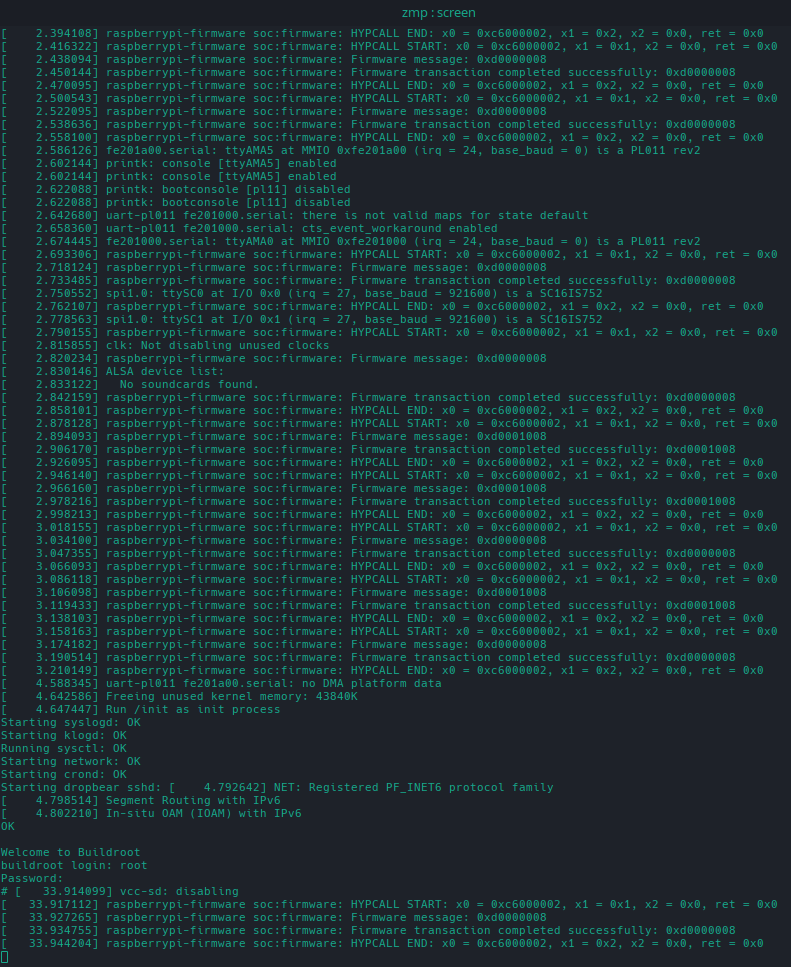
\includegraphics[width=1.0\textwidth]{./img/png/rpi-fw-validation-1}
%   \caption{PX4 VM boot}%
%   \label{fig:rpi-fw-validation-1}
%   \end{subfigure}
% %
%   \begin{subfigure}[t]{.54\textwidth}
%     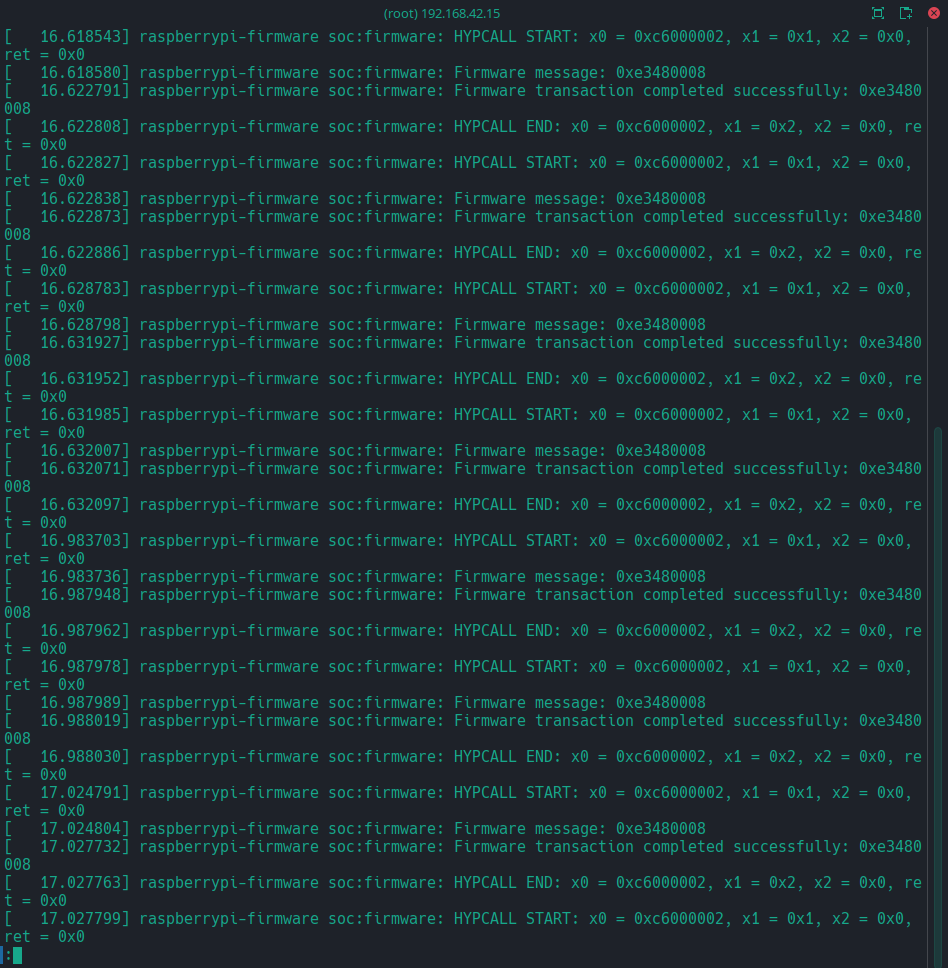
\includegraphics[width=1.0\textwidth]{./img/png/rpi-fw-validation-2}
%   \caption{Video surveillance VM boot}%
%   \label{fig:rpi-fw-validation-2}
%   \end{subfigure}
%   % 
%   \caption{Mailbox supervisor validation}%
%   \label{fig:rpi-fw-validation}
% \end{figure}

We've followed the same procedure, described in the previous section, to
\textbf{build the firmware}. Then, the \textbf{boot artifacts were deployed} to the
\gls{sd} card, namely: the firmware, the secondary bootloaders
(\lstinline{bl31.bin} and \lstinline{u-boot.bin}), the boot
configuration file (\lstinline{config.txt}), and the Bao hypervisor executable
(\lstinline{bao.bin}) containing the PX4 and video surveillance
guests. Additionally, and optionally, the guests binaries --
\lstinline{linux_1.bin} and \lstinline{linux_2.bin} -- were deployed to ease the
testing process: first each guest's binary is executed on the \gls{uavic}
platform's; if each guest is operating correctly, then we test it atop of the
Bao hypervisor.

Lastly, \textbf{we validated the \gls{sspfs} solution}, running \lstinline{bao.bin} on
the \gls{uavic} as follows:
\lstinline[language=bash]{la=0x80000; fatload mmc 0 $la bao.bin; go $la}.
To inspect the boot process of both guests we remotely accessed each one using:
(1) the debug console for the PX4 \gls{vm}
(\lstinline{screen /dev/ttyUSB0 115200}) -- Listing~\ref{lst:sspfs-boot-px4};
(2) \texttt{ssh} over Wi-Fi for the video surveillance \gls{vm}
(\lstinline{ssh root@192.168.1.X}) -- Listing~\ref{lst:sspfs-boot-cam}.

Listing~\ref{lst:sspfs-boot-px4} shows the \lstinline{bao.bin} execution (line 2),
which uses the same console that PX4 \gls{vm}. Lines 3--6 shows the Linux
\gls{os} build information. Lines 10--22 shows the memory configuration for the
\gls{cma} and \gls{dma}, and the early boot console (UART5). Lines 24--25 show
the firmware is correctly accessed by the mailbox and in lines 34--35 show the
\gls{spi} devices' initialization. Finally, line 49 shows the welcome message
from Buildroot which precedes the login.

\begin{longlisting}
\centering
\inputminted[]{kconfig}{./listing/sspfs-boot-px4.txt}
\caption{SSPFS: PX4 VM boot log (excerpt)}
\label{lst:sspfs-boot-px4}
\end{longlisting}

Listing~\ref{lst:sspfs-boot-px4} shows the remote access to the video
surveillance \gls{vm}. Lines 8--10 shows the Linux
\gls{os} build information -- the same as the one for PX4 \gls{vm}. Lines 15--30 shows the memory configuration for the
\gls{cma} and \gls{dma}. Lines 32--40 show the boot of the 3 \glspl{cpu}
allocated to this \gls{vm}.
Lines 42--43 show the firmware is correctly accessed by the mailbox, validating
once again the mailbox supervisor.
Lines 47--56 show the \gls{usb} devices enumeration, namely the camera and the
Wi-Fi dongle. Lines 58-64 show the automatic authentication in the Wi-Fi
network, provided by \texttt{iwd}. The resulting \texttt{wlan}'s network
configuration is displayed in lines 73--80, demonstrating the successful
connection to the network.

\begin{longlisting}
\centering
\inputminted[]{kconfig}{./listing/sspfs-boot-cam.txt}
\caption{SSPFS: Video surveillance VM boot log (excerpt)}
\label{lst:sspfs-boot-cam}
\end{longlisting}

After verifying both guests boot successfully, we need to analyze the execution
of the PX4 and video surveillance applications.

\textbf{FALTA PX4 application validation}

Fig.~\ref{fig:sspfs-cam-qgc} shows the video surveillance application validation
in the \gls{sspfs} system. On the top terminal we have the \lstinline{sender}'s application,
running in the \gls{uavic} (\lstinline{192.168.1.59}); in the bottom terminal
the \lstinline{receiver}'s application; and in the middle the \gls{gui} launched
by the \lstinline{receiver}, displaying the camera's live streaming to the ground station, validating the
video surveillance \gls{vm}.

\begin{figure}
  \centering
  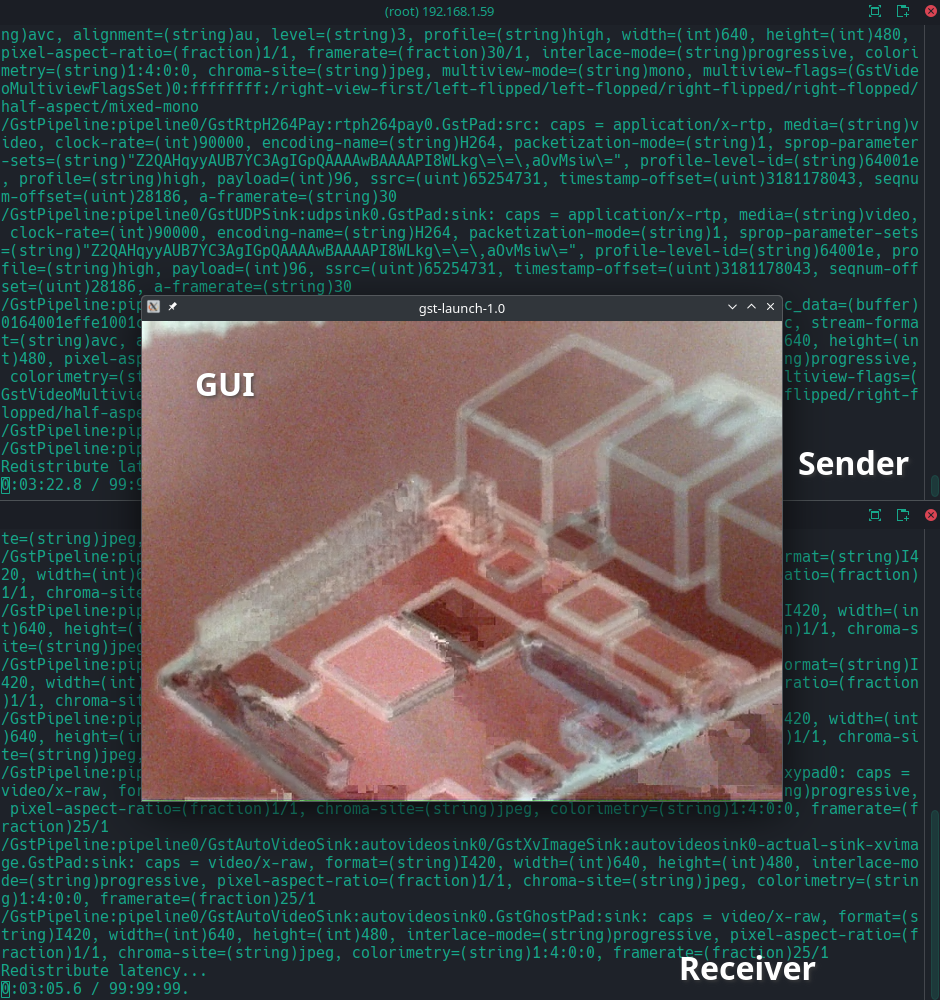
\includegraphics[width=0.8\textwidth]{./img/png/sspfs-cam-qgc} 
  \caption{SSPFS: Video surveillance application}%
  \label{fig:sspfs-cam-qgc}
\end{figure}


\section{Summary}
\label{sec:summary-implem}
In this chapter we implemented the \gls{uspfs} and \gls{sspfs}
solutions, following the overall implementation workflow. Firstly, we tested and
validated the base system: (1) we assembled the \gls{uav}; (2) build PX4 for
the target platform and used it (3) to configure the \gls{uav}; (4) setup and
validated the video surveillance pipeline running on the \gls{uavic} and the
ground station.

We then implemented the \gls{uspfs} solution by deploying an embedded custom
Linux \gls{os} image, containing the PX4 and video surveillance stacks, that
runs on the \gls{uavic} platform. We configured the system to support the device
drivers and modules required by both stacks and patched the \gls{atf} to
redirect console output to \lstinline{ttyAMA5} due to \gls{uavic}
restrictions. We also configured the boot process using U-Boot environment
script and \lstinline{config.txt} to support automatic initialization of the
\gls{uavic} platform and execution of the custom Linux \gls{os} image. We tested
the PX4 and video surveillance stacks, verifying its correct execution, which
validated the implementation.

Finally, we implemented the \gls{sspfs} solution by deploying each software
stack to a separate \gls{vm}, consisting of a custom Linux \gls{os} guest, running
atop of the Bao hypervisor. The first step was to build each guest. Then, we
built the hypervisor and the \glspl{vm}. We forked the Bao hypervisor to add
support for the custom \gls{uart} port used (\lstinline{ttyAMA5}). Next, we
created a custom Bao's configuration to describe the available resources to each
guests: PX4 is more constrained -- 1 \gls{cpu}, 144 MB of \gls{ram}, 9 devices; video
surveillance uses the remaining 3 \glspl{cpu}, 624 MB of \gls{ram}, and 4
devices. To enable mailbox sharing between guests we implemented and validalted the mailbox
supervisor in Bao, which also required patching the Raspberry Pi firmware
mailbox driver on the Linux kernel. Lastly, we validated the \gls{sspfs}
solution, running \lstinline{bao.bin} on the \gls{uavic} and inspecting the boot
process of each guest using the available debug serial port and \texttt{ssh}
over Wi-Fi. After validating the boot process, we then analyzed each software
stack behavior. We concluded PX4 and video surveillance stacks operate correctly
when running on its guest, validating the implementation of the \gls{sspfs} solution.

%%% Local Variables:
%%% mode: LaTeX
%%% TeX-master: "../template"
%%% reftex-default-bibliography: ("../Bibliography/mieeic.bib")
%%% ispell-local-dictionary: "american"
%%% End:
